% Options for packages loaded elsewhere
\PassOptionsToPackage{unicode}{hyperref}
\PassOptionsToPackage{hyphens}{url}
%
\documentclass[
  12pt,
]{article}
\title{Effective Pest Treament That Protects Pollinators}
\usepackage{etoolbox}
\makeatletter
\providecommand{\subtitle}[1]{% add subtitle to \maketitle
  \apptocmd{\@title}{\par {\large #1 \par}}{}{}
}
\makeatother
\subtitle{\url{https://github.com/shivanikuckreja/CitrolaKuckrejaSaltman_ENV872_EDA_FinalProject/tree/main/Project}}
\author{Sam Saltman, Shivani Kuckreja, Jessica Citrola}
\date{}

\usepackage{amsmath,amssymb}
\usepackage{lmodern}
\usepackage{iftex}
\ifPDFTeX
  \usepackage[T1]{fontenc}
  \usepackage[utf8]{inputenc}
  \usepackage{textcomp} % provide euro and other symbols
\else % if luatex or xetex
  \usepackage{unicode-math}
  \defaultfontfeatures{Scale=MatchLowercase}
  \defaultfontfeatures[\rmfamily]{Ligatures=TeX,Scale=1}
  \setmainfont[]{Times New Roman}
\fi
% Use upquote if available, for straight quotes in verbatim environments
\IfFileExists{upquote.sty}{\usepackage{upquote}}{}
\IfFileExists{microtype.sty}{% use microtype if available
  \usepackage[]{microtype}
  \UseMicrotypeSet[protrusion]{basicmath} % disable protrusion for tt fonts
}{}
\makeatletter
\@ifundefined{KOMAClassName}{% if non-KOMA class
  \IfFileExists{parskip.sty}{%
    \usepackage{parskip}
  }{% else
    \setlength{\parindent}{0pt}
    \setlength{\parskip}{6pt plus 2pt minus 1pt}}
}{% if KOMA class
  \KOMAoptions{parskip=half}}
\makeatother
\usepackage{xcolor}
\IfFileExists{xurl.sty}{\usepackage{xurl}}{} % add URL line breaks if available
\IfFileExists{bookmark.sty}{\usepackage{bookmark}}{\usepackage{hyperref}}
\hypersetup{
  pdftitle={Effective Pest Treament That Protects Pollinators},
  pdfauthor={Sam Saltman, Shivani Kuckreja, Jessica Citrola},
  hidelinks,
  pdfcreator={LaTeX via pandoc}}
\urlstyle{same} % disable monospaced font for URLs
\usepackage[margin=2.54cm]{geometry}
\usepackage{longtable,booktabs,array}
\usepackage{calc} % for calculating minipage widths
% Correct order of tables after \paragraph or \subparagraph
\usepackage{etoolbox}
\makeatletter
\patchcmd\longtable{\par}{\if@noskipsec\mbox{}\fi\par}{}{}
\makeatother
% Allow footnotes in longtable head/foot
\IfFileExists{footnotehyper.sty}{\usepackage{footnotehyper}}{\usepackage{footnote}}
\makesavenoteenv{longtable}
\usepackage{graphicx}
\makeatletter
\def\maxwidth{\ifdim\Gin@nat@width>\linewidth\linewidth\else\Gin@nat@width\fi}
\def\maxheight{\ifdim\Gin@nat@height>\textheight\textheight\else\Gin@nat@height\fi}
\makeatother
% Scale images if necessary, so that they will not overflow the page
% margins by default, and it is still possible to overwrite the defaults
% using explicit options in \includegraphics[width, height, ...]{}
\setkeys{Gin}{width=\maxwidth,height=\maxheight,keepaspectratio}
% Set default figure placement to htbp
\makeatletter
\def\fps@figure{htbp}
\makeatother
\setlength{\emergencystretch}{3em} % prevent overfull lines
\providecommand{\tightlist}{%
  \setlength{\itemsep}{0pt}\setlength{\parskip}{0pt}}
\setcounter{secnumdepth}{5}
\ifLuaTeX
  \usepackage{selnolig}  % disable illegal ligatures
\fi

\begin{document}
\maketitle

\newpage
\tableofcontents 
\newpage
\listoftables 
\newpage
\listoffigures 
\newpage

\hypertarget{rationale-and-research-questions}{%
\section{Rationale and Research
Questions}\label{rationale-and-research-questions}}

\textbf{Pollination is a critical component of agriculture. Bees are
important pollinators, however, a decline in pollinators has been linked
to extensive use of insecticides. Measuring hazardous and lethal
toxicity as well as potential side effects for various pollinators could
be utilized for research or management recommendations. Our analysis
evaluates if there are exposure methods and chemicals that do not cause
significant harm to bees while eliminating pests. The goal of our
analysis is to determine potential treatment methods that reduce pests
while having a non-lethal impact on bees.}

Questions:

\begin{enumerate}
\def\labelenumi{\arabic{enumi}.}
\item
  \emph{Is there an exposure type that is more likely to cause mortality
  for bees vs.~non-bee insects?}
\item
  \emph{Are there chemicals that are more likely to cause mortality for
  bees vs.~non-bee insects?}
\end{enumerate}

\newpage

\hypertarget{dataset-information}{%
\section{Dataset Information}\label{dataset-information}}

Data Source: The dataset was pulled from a repository created for
Environmental Data Analytics at Duke University in 2020. The data
collected is from several EPA studies on neonicotinoids and their
effects on insects. The data we will be analyzing is the type of
chemical administered, how it was administered, and how both of these
variables impact insects.

In the wrangling process, we selected the relevant information to our
topic. This includes the chemical type, chemical number, insect species,
lifestage and age of the species, exposure type, the effect of the
exposure and the measurement of the exposure. An example of an exposure
type is giving food to a bee. An example of an effect is mortality, and
the measurement is a more detailed analysis of the effect.

We converted all these selected categorical variables to factors to prep
for analysis. In the next step, we processed two data frames -- all bee
species and all non-bee species. The split resulted in 2529 non-bee
observations and 1407 bee observations. Lastly we added a mortality
column using an ifelse statement. We did this to run a binomial glm in
our analysis. We coded mortality as 1 and everything else as 0.

\begin{longtable}[]{@{}ll@{}}
\caption{Summary Data}\tabularnewline
\toprule
Detail & Description \\
\midrule
\endfirsthead
\toprule
Detail & Description \\
\midrule
\endhead
Data Source & EPA ECOTOX Knowledgebase \\
------- & --------- \\
Retrieved From & \url{https://cfpub.epa.gov/ecotox/help.cfm} \\
------- & --------- \\
Date Range & 1982-2019 \\
\bottomrule
\end{longtable}

\begin{longtable}[]{@{}ll@{}}
\toprule
& x \\
\midrule
\endhead
CAS.Number & factor \\
Chemical.Name & factor \\
Species.Common.Name & factor \\
Organism.Lifestage & factor \\
Organism.Age & factor \\
Exposure.Type & factor \\
Effect & factor \\
Effect.Measurement & factor \\
\bottomrule
\end{longtable}

\newpage

\hypertarget{exploratory-analysis}{%
\section{Exploratory Analysis}\label{exploratory-analysis}}

Summary of all species in study

\begin{longtable}[]{@{}lr@{}}
\caption{Species List}\tabularnewline
\toprule
& x \\
\midrule
\endfirsthead
\toprule
& x \\
\midrule
\endhead
Honey Bee & 667 \\
Parasitic Wasp & 285 \\
Buff Tailed Bumblebee & 183 \\
Carniolan Honey Bee & 152 \\
Bumble Bee & 140 \\
Italian Honeybee & 113 \\
Japanese Beetle & 94 \\
Asian Lady Beetle & 76 \\
Euonymus Scale & 75 \\
Wireworm & 69 \\
European Dark Bee & 66 \\
Minute Pirate Bug & 62 \\
Asian Citrus Psyllid & 60 \\
Parastic Wasp & 58 \\
Colorado Potato Beetle & 57 \\
Parasitoid Wasp & 51 \\
Erythrina Gall Wasp & 49 \\
Beetle Order & 47 \\
Snout Beetle Family, Weevil & 47 \\
Sevenspotted Lady Beetle & 46 \\
True Bug Order & 45 \\
Buff-tailed Bumblebee & 39 \\
Aphid Family & 38 \\
Cabbage Looper & 38 \\
Sweetpotato Whitefly & 37 \\
Braconid Wasp & 33 \\
Cotton Aphid & 33 \\
Predatory Mite & 33 \\
Ladybird Beetle Family & 30 \\
Parasitoid & 30 \\
Scarab Beetle & 29 \\
Spring Tiphia & 29 \\
Thrip Order & 29 \\
Ground Beetle Family & 27 \\
Rove Beetle Family & 27 \\
Tobacco Aphid & 27 \\
Chalcid Wasp & 25 \\
Convergent Lady Beetle & 25 \\
Stingless Bee & 25 \\
Spider/Mite Class & 24 \\
Tobacco Flea Beetle & 24 \\
Citrus Leafminer & 23 \\
Ladybird Beetle & 23 \\
Mason Bee & 22 \\
Mosquito & 22 \\
Argentine Ant & 21 \\
Beetle & 21 \\
Flatheaded Appletree Borer & 20 \\
Horned Oak Gall Wasp & 20 \\
Leaf Beetle Family & 20 \\
Potato Leafhopper & 20 \\
Tooth-necked Fungus Beetle & 20 \\
Codling Moth & 19 \\
Black-spotted Lady Beetle & 18 \\
Calico Scale & 18 \\
Fairyfly Parasitoid & 18 \\
Lady Beetle & 18 \\
Minute Parasitic Wasps & 18 \\
Mirid Bug & 18 \\
Mulberry Pyralid & 18 \\
Silkworm & 18 \\
Vedalia Beetle & 18 \\
Araneoid Spider Order & 17 \\
Bee Order & 17 \\
Egg Parasitoid & 17 \\
Insect Class & 17 \\
Moth And Butterfly Order & 17 \\
Oystershell Scale Parasitoid & 17 \\
Hemlock Woolly Adelgid Lady Beetle & 16 \\
Hemlock Wooly Adelgid & 16 \\
Mite & 16 \\
Onion Thrip & 16 \\
Western Flower Thrips & 15 \\
Corn Earworm & 14 \\
Green Peach Aphid & 14 \\
House Fly & 14 \\
Ox Beetle & 14 \\
Red Scale Parasite & 14 \\
Spined Soldier Bug & 14 \\
Armoured Scale Family & 13 \\
Diamondback Moth & 13 \\
Eulophid Wasp & 13 \\
Monarch Butterfly & 13 \\
Predatory Bug & 13 \\
Yellow Fever Mosquito & 13 \\
Braconid Parasitoid & 12 \\
Common Thrip & 12 \\
Eastern Subterranean Termite & 12 \\
Jassid & 12 \\
Mite Order & 12 \\
Pea Aphid & 12 \\
Pond Wolf Spider & 12 \\
Spotless Ladybird Beetle & 11 \\
Glasshouse Potato Wasp & 10 \\
Lacewing & 10 \\
Southern House Mosquito & 10 \\
Two Spotted Lady Beetle & 10 \\
Ant Family & 9 \\
Apple Maggot & 9 \\
(Other) & 670 \\
\bottomrule
\end{longtable}

\newpage

Bar chart comparing exposure type to mortality count of bees. It
initially looked like bees are more likely to die when chemical exposure
comes from consuming food.The other exposure types do not look
particularly significant

\begin{figure}
\centering
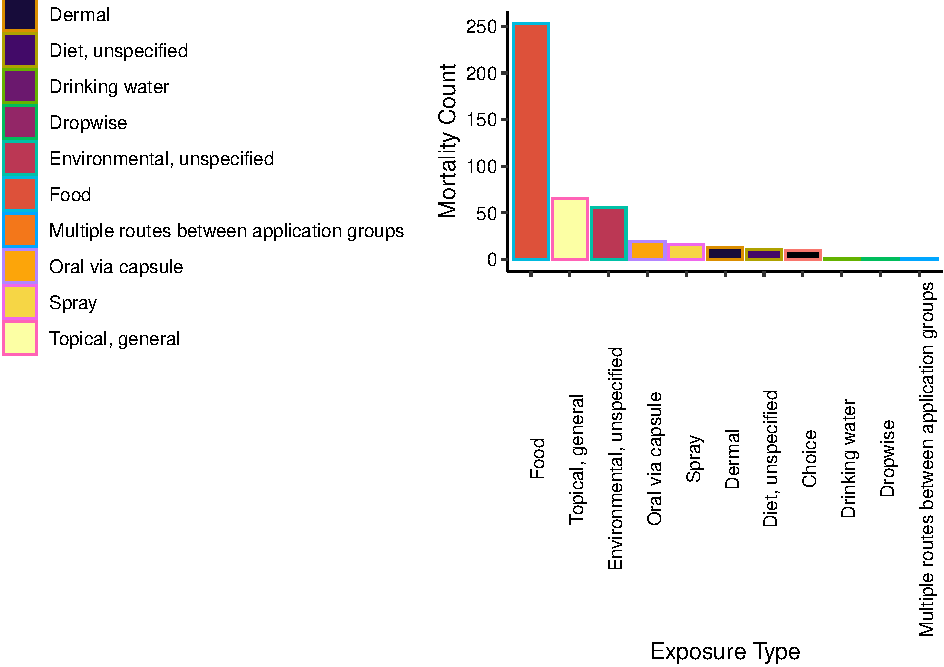
\includegraphics{UpdatedwithModel_files/figure-latex/bee exposure-1.pdf}
\caption{Bee Mortality by Exposure Type}
\end{figure}

\newpage

Bar chart comparing exposure type to mortality count of non-bees.
Exposure from an environmental source appears more lethal to non-bees
species.

\begin{figure}
\centering
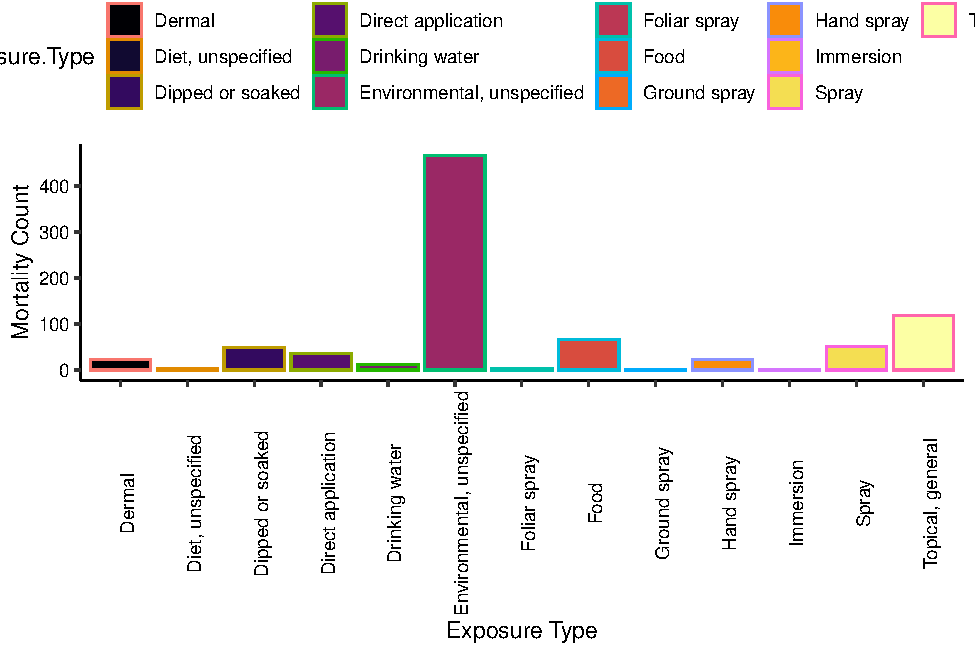
\includegraphics{UpdatedwithModel_files/figure-latex/non bee exposure-1.pdf}
\caption{Non-bee Mortality by Exposure Type}
\end{figure}

\newpage

The next area of exploration was looking into how many bee and non-bee
samples died from exposure to certain chemical compounds. We used the
chemical number as the chemical names are complex.

This bar chart looking at bees suggests that three types of chemical
compounds in this dataset are toxic to bees.

\begin{figure}
\centering
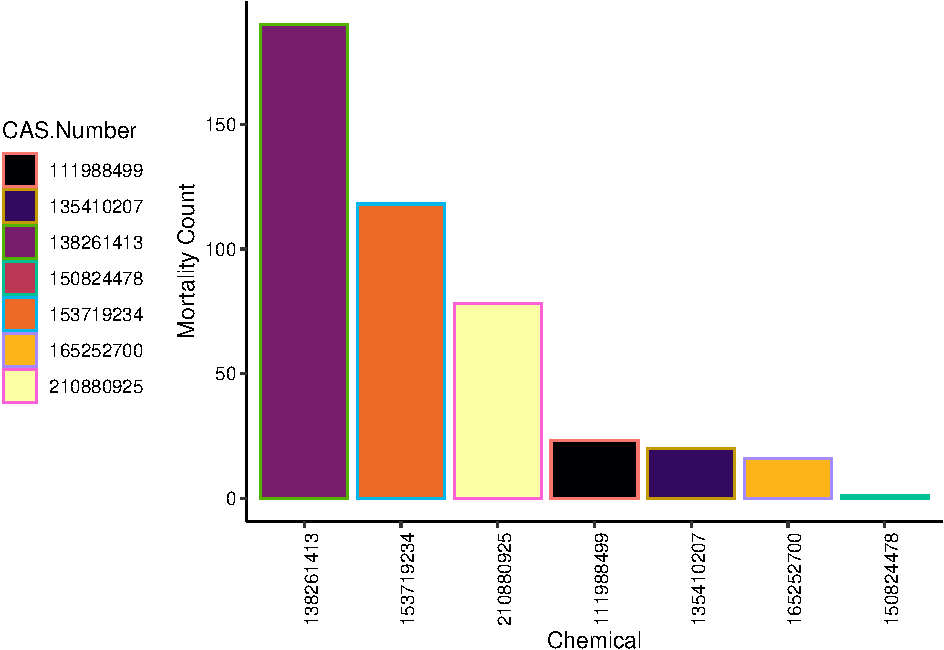
\includegraphics{UpdatedwithModel_files/figure-latex/bee chemical-1.pdf}
\caption{Bee Mortality by Chemical}
\end{figure}

\newpage

This bar chart looking at bees suggests that three types of chemical
compounds in this dataset are toxic to non-bees.

\begin{figure}
\centering
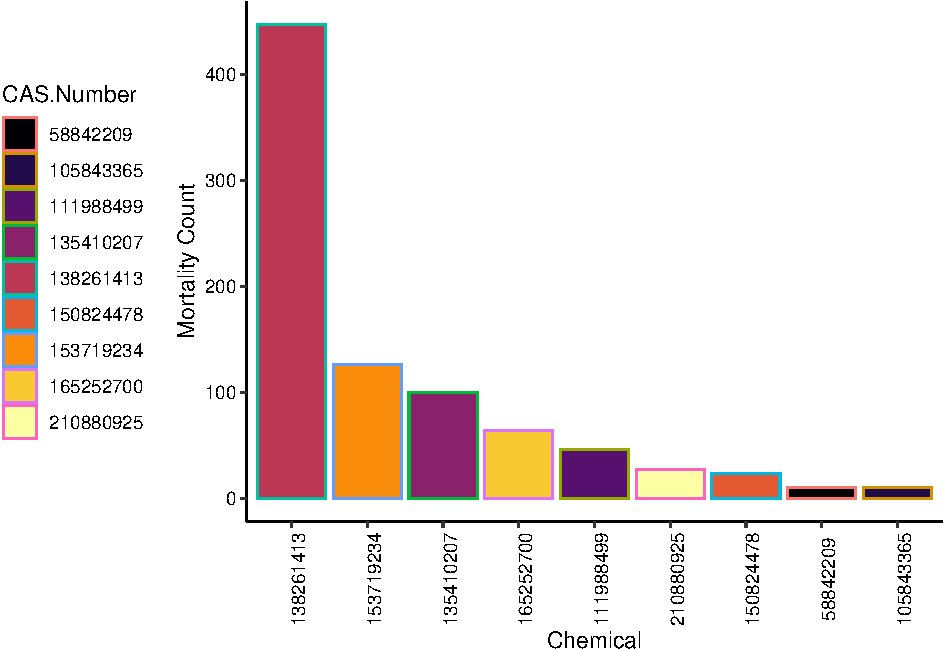
\includegraphics{UpdatedwithModel_files/figure-latex/non bee chemical-1.pdf}
\caption{Non-bee Mortality by Chemical}
\end{figure}

Next we analyze to see if there is any statistical significance
supporting these observations. \newpage

\hypertarget{analysis}{%
\section{Analysis}\label{analysis}}

We ran GLMs to analyze our categorical data. Using the if/else statement
to create the mortality column, we were able to compare mortality
against all other effects. We ran two GLMs for the bee category and two
for the non-bee categories. The two types of GLMs we ran analyzed
mortality against exposure type and mortality against chemical type.To
understand if this regression was a fit, we ran a pseudo regression
using the pR2 function on each GLM as well

The `logit' model evaluated the effect of exposure type on mortality on
bee species. The results of this model showed that topical exposure had
a significant effect on bee mortality (p=.009). For every one unit
change in topical, the odds of mortality increase by 1.1787. In
comparison to non-bee species, `logit2' had various exposure types that
had a significant effect on mortality. The significant exposure types
included dipped or soaked, direct application, drinking water,
environmental (unspecified), foliar spray, ground spray, hand spray,
spray, and topical.

The `logit3' and `logit4' models evaluated which chemical types have a
lethal effect on bee and non bee species. The results of `logit3' showed
that nearly all chemical types with data had a significant effect on
bees. However, the only chemical that was not significant (150824478)
only had one entry. The results of `logit4' showed that no chemical had
a significant effect on non-bee species. The results of the four models
are summarized in the tables below.

We evaluated the goodness-of-fit by finding the McFadden pseudo
R-squared for each model. The model for exposure type and non-bee
mortality (`logit2') had a good fit with a McFadden pseudo R-squared
value of .214. However, the rest of the models had very low pseudo
R-squared values. As a result, these models may not provide the most
predictive information.

\hypertarget{question-1-is-there-an-exposure-type-that-is-more-likely-to-cause-mortality-for-bees-vs.-non-bee-insects}{%
\subsection{Question 1: Is there an exposure type that is more likely to
cause mortality for bees vs.~non-bee
insects?}\label{question-1-is-there-an-exposure-type-that-is-more-likely-to-cause-mortality-for-bees-vs.-non-bee-insects}}

\textbf{Results of Statistical Analysis on Exposure Type and Mortality
on Bees}

\begin{longtable}[]{@{}ll@{}}
\toprule
Exposure Effect on Bees & Pr(\textgreater{} \\
\midrule
\endhead
Topical, general & 0.009 ** \\
\bottomrule
\end{longtable}

*Pseudo McFadden Score = 0.07748671

\textbf{Results of Statistical Analysis on Exposure Type and Mortality
on Non-bees}

\begin{longtable}[]{@{}ll@{}}
\toprule
Non-Bee Exposure Type & Pr(\textgreater{} \\
\midrule
\endhead
Dipped or soaked & 0.003227 \\
Direct application & 3.42e-05 \\
Drinking water & 0.021404 \\
Environmental, unspecified & 0.000278 \\
Foliar spray & 3.14e-11 \\
Ground spray & 1.15e-06 \\
Hand spray & 3.41e-09 \\
Spray & 2.16e-08 \\
Topical, general & 0.018538 \\
\bottomrule
\end{longtable}

*Pseudo McFadden Score = 0.2142859

\hypertarget{question-2-are-there-chemicals-that-are-more-likely-to-cause-mortality-for-bees-vs.-non-bee-insects}{%
\subsection{Question 2: Are there chemicals that are more likely to
cause mortality for bees vs.~non-bee
insects?}\label{question-2-are-there-chemicals-that-are-more-likely-to-cause-mortality-for-bees-vs.-non-bee-insects}}

\textbf{Results of Statistical Analysis on Chemical Types and Mortality
on Bees}

\begin{longtable}[]{@{}ll@{}}
\toprule
Chemical Effect on Bees & Pr(\textgreater{} \\
\midrule
\endhead
135410207 & 9.10e-06 *** \\
138261413 & 6.39e-07 *** \\
153719234 & 0.017062 * \\
165252700 & 0.003599 ** \\
210880925 & 0.000189 *** \\
\bottomrule
\end{longtable}

*Pseudo McFadden Score = 0.03867201

\textbf{Results of Statistical Analysis on Chemical Types and Mortality
on Non-bees}

\begin{longtable}[]{@{}ll@{}}
\toprule
Chemical Effect on Non-Bees & Pr(\textgreater{} \\
\midrule
\endhead
Chemical & None \\
\bottomrule
\end{longtable}

*Pseudo McFadden Score = 4.373360e-02

\newpage

\hypertarget{summary-and-conclusions}{%
\section{Summary and Conclusions}\label{summary-and-conclusions}}

We found that the exposure technique influenced the mortality
predictiveness of the neonicotinoids on the species in our dataset. Our
model showed that topical exposure had a significant effect on mortality
for bee species, but the pseudo R-squared suggests that the model might
not be a good fit to the data. Our model for exposure techniques on non
bee species shows that several exposure techniques significantly
affected mortality. The pseudo R-squared value of .214 suggests that
this model is a good fit. Regarding the data on chemical types, our
models showed that no chemical had a significant effect on non-bee
species mortality. For bee species, we did find several chemical types
that had a significant effect on mortality, but this model also had a
low pseudo R-squared and may not be the most predictive for our data.
Given our data on exposure types and their effects on bee and non-bee
mortality, we suggest that spray exposure techniques could maximize the
effectiveness on reducing unwanted pests while preventing mortality on
bees.

\newpage

\hypertarget{appendix}{%
\section{Appendix}\label{appendix}}

\begin{figure}
\centering
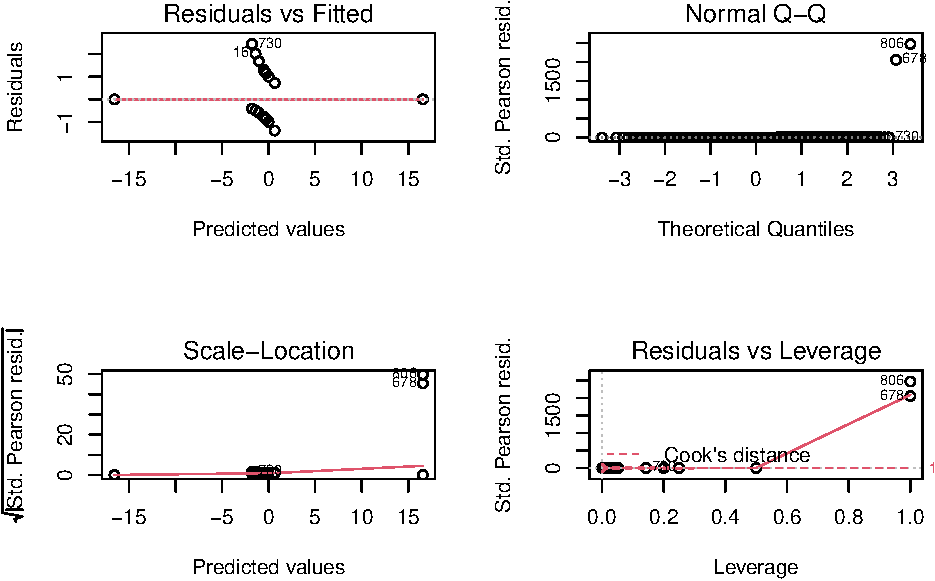
\includegraphics{UpdatedwithModel_files/figure-latex/unnamed-chunk-8-1.pdf}
\caption{Residual Plot for Bee Mortality by Exposure Type}
\end{figure}

\newpage

\begin{figure}
\centering
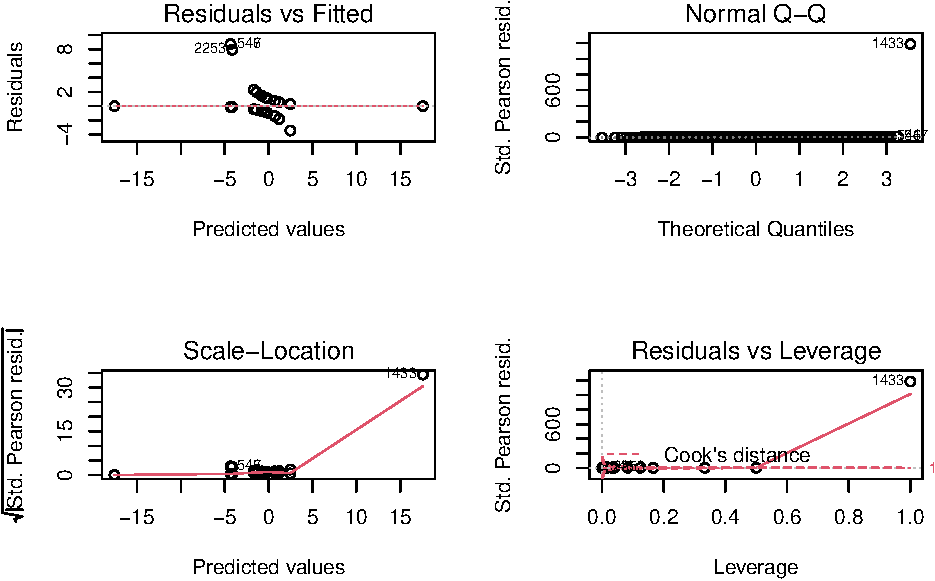
\includegraphics{UpdatedwithModel_files/figure-latex/unnamed-chunk-9-1.pdf}
\caption{Residual Plot for Non-Bee Mortality by Exposure Type}
\end{figure}

\newpage

\begin{figure}
\centering
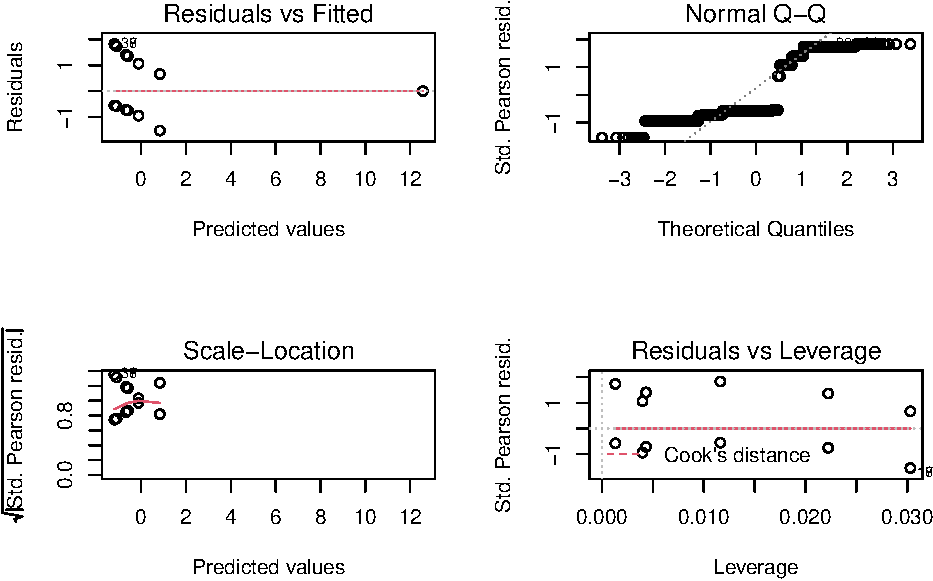
\includegraphics{UpdatedwithModel_files/figure-latex/unnamed-chunk-10-1.pdf}
\caption{Residual Plot for Bee Mortality by Chemical Type}
\end{figure}

\newpage

\begin{figure}
\centering
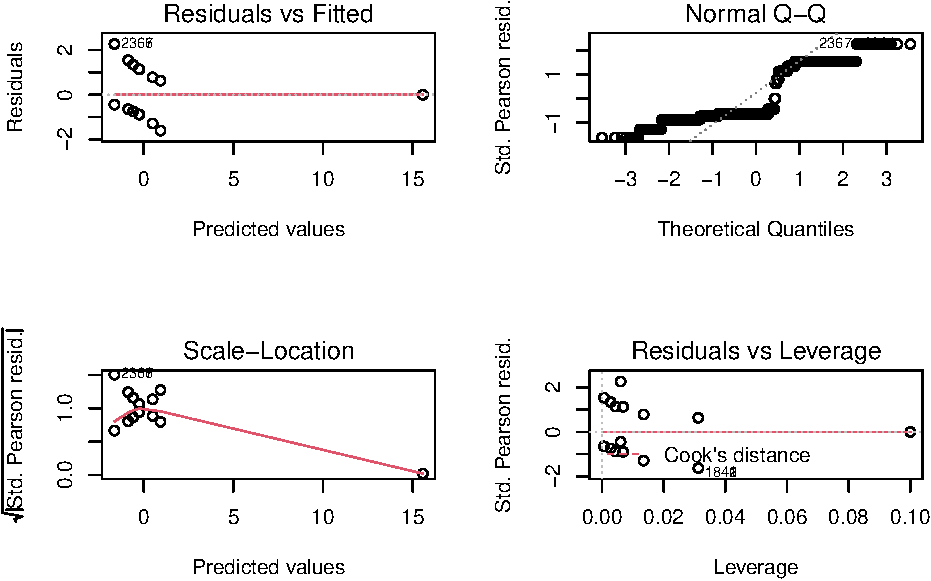
\includegraphics{UpdatedwithModel_files/figure-latex/unnamed-chunk-11-1.pdf}
\caption{Residual Plot for Non-Bee Mortality by Chemical Type}
\end{figure}

\end{document}
